\documentclass[11pt,a4paper]{article}

% ── Packages ──────────────────────────────────────────────
\usepackage[utf8]{inputenc}
\usepackage[T1]{fontenc}
\usepackage{lmodern}
\usepackage[margin=0.75in]{geometry}
\usepackage{amsmath,amssymb}
\usepackage{graphicx}
\usepackage{booktabs}
\usepackage{longtable}
\usepackage{hyperref}
% \usepackage{cleveref}  % disabled due to MiKTeX First Aid conflict
\usepackage{setspace}
\usepackage{parskip}
\usepackage[nottoc]{tocbibind}
\usepackage{csquotes}
\usepackage{tabularx}
\usepackage{array}
\usepackage[font=small,labelfont=bf]{caption}
\usepackage{fancyhdr}

\hypersetup{
  colorlinks=true,
  linkcolor=blue,
  citecolor=blue,
  urlcolor=blue
}

\setstretch{1.05}

% ── Header setup ─────────────────────────────────────────
\pagestyle{fancy}
\fancyhf{}
\fancyhead[L]{Krishnasree Kelath}
\fancyhead[R]{Student ID: 2540124}
\fancyfoot[C]{\thepage}
\renewcommand{\headrulewidth}{0.4pt}

% ── Document begins ──────────────────────────────────────
\begin{document}

% ── Title + Name ─────────────────────────────────────────
\begin{center}
{\LARGE\bfseries How Do We Hear a \textit{Raga}?\par}
\vspace{0.4cm}
{\Large\bfseries An Interpretable Cognitive Model of Melodic Recognition\par}
\vspace{0.3cm}
{\large Krishnasree Kelath \quad (Student ID: 2540124)\par}
{\large School of Computer Science -- University of Birmingham\par}
{\large Supervisor: Martin Escardo\par}
\end{center}

\vspace{0.3cm}

% ── Abstract ──────────────────────────────────────────────
{\small
\noindent\textbf{Abstract.}
Music recognition systems typically analyse acoustic and spectral features: timbral content, signal characteristics, raw audio representations. In Carnatic music, however, identity is governed by the \textit{raga}: a melodic grammar of characteristic phrases, note hierarchies, and ornamentation that defines how a piece is recognised. Existing \textit{raga} recognition systems either treat this as a generic classification problem or use pitch-level features that capture only a subset of the cues listeners rely on, and none connects its representations to models of how listeners actually perceive melodic structure. This project bridges that gap with a six-stage interpretable pipeline (pitch extraction, tonic estimation, swara mapping, and feature extraction) in which every feature dimension has a cognitive or musicological interpretation. Under GroupKFold cross-validation on the SARAGA Carnatic dataset (46 tracks, 13 \textit{ragas}, 1,648 segments after excluding catastrophic tonic failures), an SVM using just 16 dwell-time and v\=adi features achieves 67.8\% weighted F1 (69.6\% track accuracy), outperforming timbral features (MFCCs) by over 63 percentage points in weighted F1. Six hypotheses test whether the features that best classify \textit{ragas} computationally are the same ones that cognitive theory predicts listeners rely on; five confirm this alignment, and the one that fails does so for musicologically predictable reasons.
\vspace{0.2cm}
% ── 1. Introduction ───────────────────────────────────────
\section{Introduction}

When a trained listener hears the opening phrases of a Carnatic performance, they can often identify the \textit{raga} within seconds. Carnatic music is one of the oldest living classical traditions, with \textit{raga}, the melodic framework governing a performance, serving as its central organising principle. This recognition does not depend on the performer's voice or instrument, but on the melodic grammar itself: which notes are emphasised, which phrases recur, and how ornamentation shapes the contour. Understanding this recognition process computationally is valuable not only for music information retrieval, but for connecting centuries of music theory to modern models of auditory cognition. Yet existing systems either achieve accuracy without explanation, or explain only a fragment of what listeners perceive. The question of how this recognition occurs sits at the intersection of three fields: the music theory that defines what a \textit{raga} is, the cognitive science that explains how humans perceive melodic patterns, and the machine learning that attempts to replicate this task computationally.

Most existing computational approaches to \textit{raga} recognition treat it as a standard audio classification problem. Deep learning systems operate on spectrograms or time-delay embeddings, achieving competitive accuracy but offering no insight into why a particular \textit{raga} was identified~\cite{gulati2016}. Simpler approaches based on pitch distributions~\cite{koduri2012} capture tonal structure but discard the sequential and durational cues that listeners rely on. Neither family of approaches explicitly connects its feature representations to models of human melodic cognition.

This project takes a different approach, guided by a central research question:

\begin{quote}
\textbf{\textit{Are the features that cognitive theory predicts listeners rely on the same features that best classify \textit{ragas} computationally?}}
\end{quote}

\noindent Answering this requires drawing on three disciplines simultaneously: Carnatic music theory defines what a \textit{raga} \textit{is}, cognitive science explains how listeners \textit{perceive} it, and machine learning provides the framework to \textit{test} whether these accounts converge. The project is structured around these three complementary pillars.

\subsection{The Three Pillars: Music, Cognition, Machine Learning}

\textbf{Musical.} \textit{Ragas} are not merely scales. Two \textit{ragas} may share identical note sets yet be recognised as entirely distinct, because \textit{raga} identity is encoded in melodic grammar: characteristic phrases (\textit{pakad}), ornamental movements (\textit{gamaka}), and note hierarchies (\textit{vadi}/\textit{samvadi}). Any computational representation must capture this grammar, not just the inventory of notes.

\textbf{Cognitive.} Listeners perceive melody through categorical pitch perception~\cite{burns1978}, tonal hierarchies~\cite{castellano1984}, and statistical learning of note transitions~\cite{tillmann2000}. An interpretable system should mirror these mechanisms, and its successes and failures should be interpretable through them.

\textbf{Machine Learning.} The system must be evaluated with methodological rigour. Cross-performance validation (GroupKFold by track) ensures that the classifier learns \textit{raga}-level patterns rather than recording-specific artefacts~\cite{sturm2014}. Comparison against both a deep learning baseline (BiLSTM) and a timbral baseline (MFCC) establishes what the interpretable features gain and what they sacrifice. Six hypotheses (H1--H6) formalise the expected relationships between feature performance and cognitive theory, transforming the evaluation from a simple accuracy comparison into a test of cognitive claims.

Each design decision, each feature, and each result in this report is examined from all three perspectives. The central finding is that the features predicted by cognitive theory, trigram sequences and dwell-time profiles, are indeed the features that best classify \textit{ragas}, while their failures align with predicted musicological boundaries. Specifically, this project contributes:

\begin{enumerate}
  \item A six-stage interpretable pipeline for Carnatic \textit{raga} recognition from audio, processing raw recordings through pitch extraction, tonic estimation, swara mapping, feature extraction, and classification.
  \item A 216-dimensional feature representation in which every dimension has a cognitive or musicological interpretation, combining trigram patterns (encoding characteristic phrases) with dwell-time profiles (encoding note prominence).
  \item Empirical evidence that melodic-structure features outperform timbral features (MFCCs) by over 63 percentage points and a BiLSTM baseline by over 31 percentage points in weighted F1 under cross-track generalisation via GroupKFold.
  \item A hypothesis-driven evaluation framework (H1--H6) linking classification results to specific claims from music cognition, with five confirmed and one yielding an informative negative.
  \item Statistical evidence that classifier confusion follows musicological kinship: within-family confusion is $5.19\times$ higher than between-family confusion ($p < 0.0001$), demonstrating that the model's error structure mirrors \textit{raga} taxonomy.
\end{enumerate}

\noindent Generative AI tools were used to assist with report drafting and code debugging for clarity in the report; all technical decisions, experimental design, and analysis are entirely self-written. An extended appendix with additional figures, per-\textit{raga} feature visualisations, all confusion matrices, and negative experiment results accompanies this report.\footnote{Appendix: \href{https://git.cs.bham.ac.uk/projects-2025-26/kxk224/-/blob/main/FinalReport/EXTENDED_APPENDIX.pdf}{https://git.cs.bham.ac.uk/projects-2025-26/kxk224/-/blob/main/FinalReport/EXTENDED\_APPENDIX.pdf}}

% ── 2. Background ─────────────────────────────────────────
\section{Background and Literature Review}

This section reviews the three bodies of literature that underpin this project. Section~\ref{sec:raga-structure} introduces the musical structures that define \textit{raga} identity. Section~\ref{sec:cognitive} examines how listeners perceive these structures cognitively. Section~\ref{sec:computational} surveys computational approaches to \textit{raga} recognition and identifies the interpretability gap this project addresses.

\subsection{\textit{Raga}: Structure, Grammar, and Identity}
\label{sec:raga-structure}

A \textit{raga} in Carnatic music is not simply a scale: two \textit{ragas} may share identical note sets yet be recognised as entirely distinct~\cite{viswanathan2004}. The Carnatic system organises \textit{ragas} into 72 parent scales (melakarta \textit{ragas}). \textit{Ragas} within the same family share the same notes, but differ in the order they are performed, the phrases that characterise them, and the relative emphasis placed on each note---making them musically related but perceptually distinct. \textit{Raga} identity emerges from melodic grammar---characteristic phrases (\textit{pakad}), short melodic motifs that function as a \textit{raga}'s signature, much as a few words can identify a language; ornamental pitch movements (\textit{gamaka}), continuous glides and oscillations between notes that give each swara its expressive shape rather than reducing it to a fixed frequency~\cite{krishnaswamy2003,krishna2012}; and a note hierarchy in which the dominant note (\textit{v\=adi}) receives the greatest emphasis through duration and frequency of occurrence, along with its sub-dominant counterpart (\textit{samv\=adi}). Any system that reduces pitch to discrete categories necessarily discards some gamaka information---a trade-off examined throughout this project.

\subsection{Cognitive Foundations of Melodic Perception}
\label{sec:cognitive}

Research in music cognition identifies several mechanisms through which listeners process melody, each of which suggests a corresponding computational representation.

\textbf{Statistical learning.} Saffran et al.~\cite{saffran1996} demonstrated that infants can segment continuous speech using only transitional probabilities between syllables. Saffran et al.~\cite{saffran1999} extended this to tone sequences, showing that both adults and infants learn recurring three-tone patterns from continuous musical streams. This provides the cognitive foundation for the trigram features in this project. Tillmann et al.~\cite{tillmann2000} further showed that such learning occurs through passive exposure, supporting statistical learning as a domain-general mechanism for acquiring musical structure. Pearce and Wiggins~\cite{pearce2012} formalised this with IDyOM, a variable-order n-gram model that predicts melodic expectation from distributional statistics---the computational analogue of the trigram representations used here.

\textbf{Tonal hierarchies.} Castellano et al.~\cite{castellano1984}, building on Krumhansl's framework of tonal cognition~\cite{krumhansl1990}, used the probe-tone method on 10 North Indian \textit{ragas} with both Indian and Western listeners. Critically, listener ratings correlated with tone duration distributions: notes played more often and for longer were perceived as more structurally important. This provides direct behavioural evidence for the dwell-time features used in this project. The study also showed that \textit{ragas} from the same th\=at cluster together perceptually---predicting that classifier confusion should follow musicological kinship.

\textbf{Categorical pitch perception.} Burns and Ward~\cite{burns1978} established that humans quantise continuous frequencies into discrete note categories, providing the cognitive basis for the swara-mapping stage.

\textbf{Cognitive parsimony.} Gigerenzer et al.~\cite{gigerenzer1999} demonstrated that simpler models using fewer cues can outperform complex models in noisy environments, a prediction tested by H3.

\textbf{Modular music processing.} Peretz and Coltheart~\cite{peretz2003} proposed that pitch organisation and timbre are handled by separate neural pathways, predicting that timbral features (MFCCs) should be uninformative for \textit{raga} classification (H2).

\subsection{Computational Approaches and the Interpretability Gap}
\label{sec:computational}

Chordia and Rae~\cite{chordia2007} demonstrated that pitch class dyad distributions---capturing which note follows which---outperform simple note inventories for \textit{raga} classification. Koduri et al.~\cite{koduri2012} extended this to Carnatic music within the CompMusic project. These methods are interpretable but discard sequential and temporal information beyond adjacent pairs. At the other extreme, Gulati et al.~\cite{gulati2016} applied deep convolutional networks to time-delay melody surfaces, achieving state-of-the-art accuracy but operating as a black box. More recently, Singh and Arora~\cite{singh2024} applied post-hoc explainability to neural networks, but the interpretability is applied after the fact to opaque representations rather than built into feature design.

A critical methodological concern was raised by Sturm~\cite{sturm2014}, who demonstrated that many MIR systems inadvertently learn recording-specific artefacts rather than musical content, motivating the cross-track generalisation via GroupKFold used in this project.

No existing system satisfies all three requirements simultaneously: (1)~features individually interpretable through a cognitive or musicological lens, (2)~evaluation that prevents artefact learning, and (3)~a hypothesis-driven framework linking feature performance to predictions from perceptual theory. This project addresses that gap.

% ── 3. Design and Implementation ──────────────────────────
\section{Design and Implementation}

This section describes the system architecture, from dataset selection through to classification. The central design principle is that every stage mirrors a cognitive or musicological process: pitch extraction corresponds to auditory processing, swara mapping to categorical perception, feature extraction to the perceptual cues reviewed in Section~\ref{sec:cognitive}, and classification to the recognition decision. All mathematical definitions underlying the pipeline (cents conversion, octave folding, circular distance, harmonic tonic scoring, weighted F1, and the permutation test) are provided in the Appendix (A). A full pipeline architecture diagram is also provided in the Appendix (B, Figure~5).

\subsection{Dataset: SARAGA Carnatic}

This project uses the SARAGA Carnatic dataset~\cite{srinivasamurthy2021}, accessed via the mirdata Python library. From 249 recordings, 89 have \textit{raga} metadata and 73 are usable after excluding tracks without ground-truth tonic annotations and multi-\textit{raga} orchestrations (\textit{raga}m\=alik\=a). These 73 tracks span 14 \textit{ragas} with substantial class imbalance (14.6:1 ratio between the largest and smallest class; see Appendix~B, Figure~6 for the full dataset distribution). Alternative datasets were considered but SARAGA prevailed due to existing CompMusic projects and presence of raga labels and full audios.

\textbf{Stage~1: Preprocessing.} Audio is loaded at 22,050~Hz, normalised, and trimmed to remove leading and trailing silence. Each track is segmented into 45-second clips with a 15-second hop (66.7\% overlap); the 45-second window ensures sufficient melodic content for stable trigram distributions (${\sim}200$ tokens), while the 15-second hop increases training data without causing data leakage under GroupKFold, producing 4,487 raw segments. Before classification (Stage~6), a voiced ratio filter at 0.25 removes segments dominated by percussion and drone, leaving 2,107 segments.

\textbf{Stage~2: Pitch extraction.} CREPE~\cite{kim2018} was selected as the primary pitch tracker because it achieves substantially lower raw pitch error than traditional methods on non-Western vocal music, where heavy ornamentation (gamaka) causes rapid pitch variation that challenges autocorrelation-based approaches like pYIN~\cite{mauch2014}. The 0.5 confidence threshold follows CREPE's recommended default. On CPU, the pipeline falls back to pYIN~\cite{mauch2014}. Representative F0 contour and voicing confidence diagnostics are in the Appendix (C, Figures~7--8).

\textbf{Stage~3: Tonic estimation.} A pitch-class histogram scored by Sa mass plus half Pa mass estimates the tonic from the range 80--300~Hz in 10-cent steps, with octave correction. This achieves 82.2\% accuracy within 50 cents; 13 mis-estimated tracks ($>50$ cents error) are excluded from primary evaluation, since a wrong tonic produces meaningless swara labels. The root cause is that CREPE locks onto the accompanying violin or v\=\i{}n\=a, whose Pa is often louder than the vocalist's Sa in mixed audio. Multiple alternative strategies were explored to improve this ceiling---including harmonic triad scoring, ensemble methods, segment-level majority voting, and source separation via Demucs and HPSS---but none surpassed 82.2\%, confirming that polyphonic audio without vocal isolation represents a hard limit (per-method error histograms, the head-to-head method comparison chart, and tonic experiment results are in the Appendix~D, Figures~9--13; HPSS and Demucs source separation experiments are detailed in Section~H.1--H.2). Their impact is quantified in the tonic ablation (Section~\ref{sec:tonic-ablation}).

\textbf{Stage~4: Swara mapping.} Each voiced pitch frame is mapped to the nearest of 12 equal-tempered swara bins (100 cents apart) if the distance falls within a tolerance of 40 cents---slightly less than a half-semitone, chosen to accommodate pitch drift in CREPE estimates while preventing adjacent swaras from overlapping. At this threshold, approximately 28\% of voiced frames are classified as glide, consistent with heavy gamaka ornamentation in Carnatic music. A temporal smoothing step converts runs shorter than 100~ms (${\sim}10$ CREPE frames) to glide, suppressing pitch estimation noise.

\begin{figure}[ht]
\centering
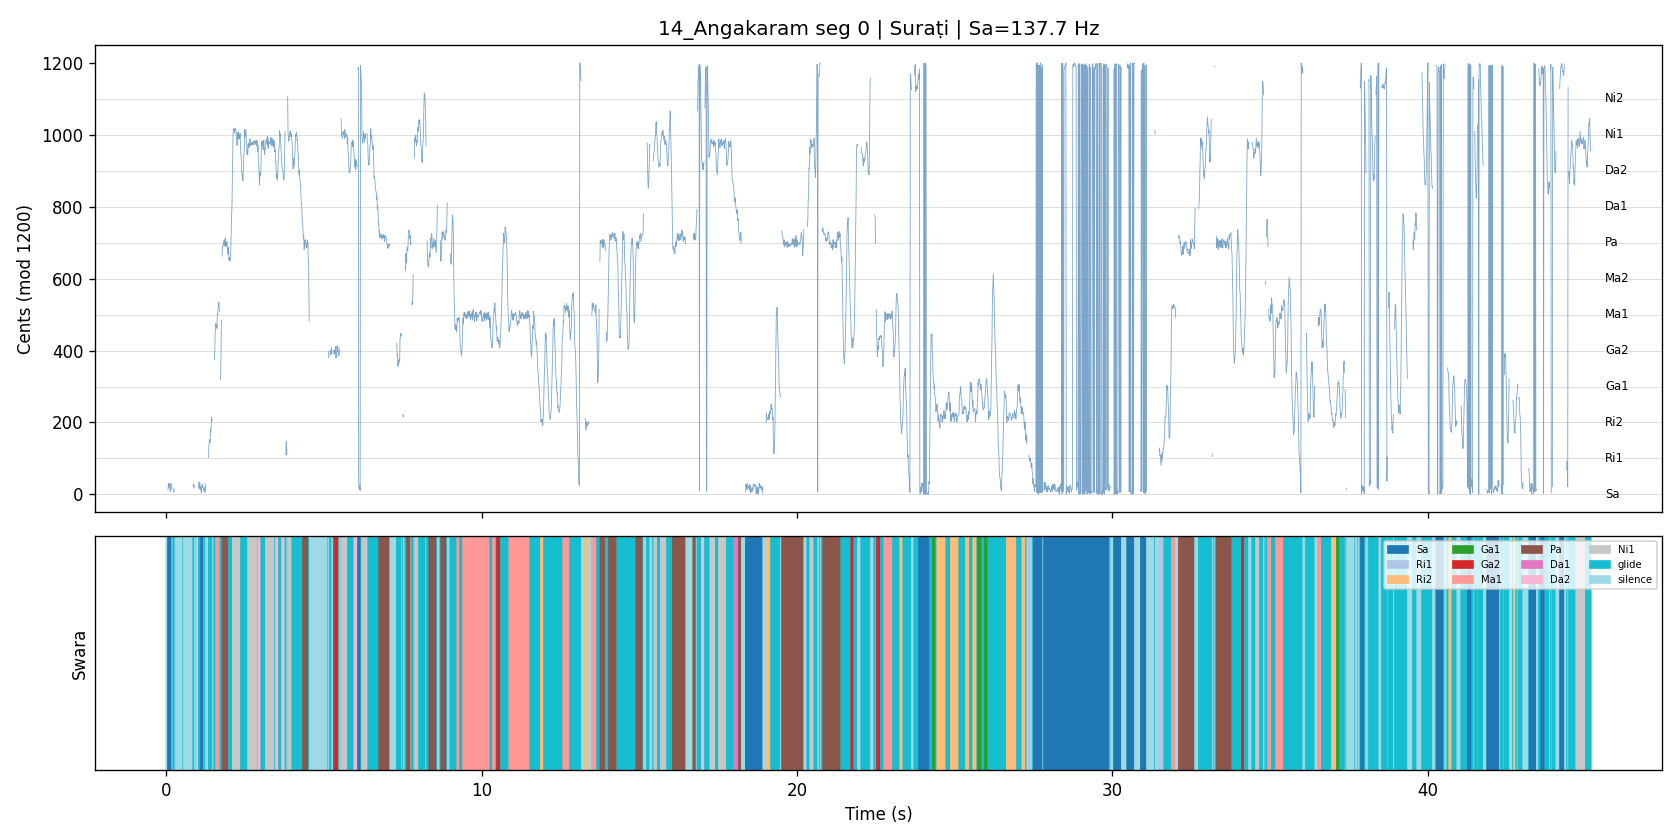
\includegraphics[width=0.85\textwidth]{outputs/figures/swara_debug/14_Angakaram__00000_swara.png}
\caption{Swara mapping for a Sura\d{t}i segment (Sa~=~137.7~Hz). Top: CREPE pitch contour in cents relative to estimated tonic, with swara bin labels (right axis). Bottom: categorical swara assignments colour-coded by pitch class; grey regions indicate gamaka glides outside the 40-cent tolerance. The continuous-to-categorical transformation illustrates the cognitive mechanism of categorical pitch perception~\cite{burns1978}. Additional swara mapping diagnostics for other tracks are in the Appendix (E, Figures~14--15).}
\label{fig:swara-debug}
\end{figure}

\textbf{Stage~5: Feature extraction.} Seven feature families are computed from the swara sequence and the underlying audio, producing multiple representations detailed in Section~\ref{sec:features}.

\textbf{Stage~6: Classification.} An SVM with RBF kernel and balanced class weights is trained using GridSearchCV, scored by weighted F1. GroupKFold with 5 folds ensures all segments from a single track appear in the same fold, preventing within-track data leakage~\cite{sturm2014}. Track-level predictions are obtained via majority voting across segment predictions. A bidirectional LSTM baseline (2 layers, 64 hidden units, 32-dim embedding, same GroupKFold splits) establishes whether hand-crafted features outperform learned sequence representations under identical data constraints. Classification and evaluation design is detailed in Section~\ref{sec:eval-design}.

\subsection{Feature Design: Mapping Pipeline to Cognition}
\label{sec:features}

Table~\ref{tab:features} presents the feature families, their dimensionality, and their cognitive analogues. This mapping is central to the project's interpretability claim: every feature dimension corresponds to a specific aspect of how humans perceive melody.

Before trigram extraction, the raw swara sequence undergoes \textit{token collapse}: consecutive runs of the same swara label are reduced to a single token, and silence and glide frames are removed. This mirrors how listeners encode melodic contour separately from rhythm~\cite{peretz2003}, but explicitly discards duration information (captured separately by dwell features) and continuous gamaka detail. The Harik\=ambh\=oji family's high within-family confusion (Section~\ref{sec:perraga}) is a direct consequence: those \textit{ragas} are distinguished precisely by the gamaka contour that token collapse discards.

\begin{table}[ht]
\centering
\caption{Feature families with their dimensionality, description, and cognitive analogues.}
\label{tab:features}
\small
\begin{tabularx}{\textwidth}{@{}llXX@{}}
\toprule
\textbf{Feature} & \textbf{Dims} & \textbf{What it captures} & \textbf{Cognitive analogue} \\
\midrule
Trigram & 200 & Top-200 three-swara sequence frequencies & Pakad recognition via statistical learning (H1) \\
Dwell/v\=adi & 16 & Mean duration per swara (12) + v\=adi/samv\=adi emphasis (4) & Note prominence hierarchy (H5) \\
PCD & 120 & Pitch class distribution (10-cent bins) & Tonal hierarchy~\cite{castellano1984} \\
Transition & 144 & Row-normalised $12\times12$ swara flow matrix & Implicit learning~\cite{tillmann2000} \\
Directional & 288--552 & Separate ascending/descending PCDs + transitions & \=Arohana/avarohana distinction (H6) \\
Auxiliary & 10 & Gamaka stats: glide ratio, transition entropy, token rate & Ornamental sensitivity \\
MFCC & 58 & Spectral envelope (20 MFCCs $\times$ 2 + chroma + spectral) & Control; should fail (H2) \\
\bottomrule
\end{tabularx}
\end{table}

\textbf{Trigrams (200d).} After token collapse, all three-swara subsequences are counted against the top 200 most frequent trigrams across the corpus. Trigrams encode pakad---the characteristic phrases that define each \textit{raga}---implementing the statistical learning mechanism documented by Saffran et al.~\cite{saffran1996,saffran1999}. The vocabulary size of 200 was chosen from 1,728 possible trigrams ($12^3$) as the point beyond which counts become too sparse given ${\sim}2{,}100$ training segments.

\textbf{Dwell/v\=adi (16d).} The v\=adi and samv\=adi are operationally defined as the swara with the highest and second-highest total frame duration per segment---an empirical proxy for the musicological concept of dominant and sub-dominant notes. Twelve dimensions record the mean duration each swara is sustained per segment. Four additional dimensions encode the v\=adi index, v\=adi fraction, samv\=adi index, and samv\=adi fraction. This captures the note prominence hierarchy that Castellano et al.~\cite{castellano1984} found to correlate with listener ratings of tonal stability.

\textbf{MFCC (58d).} Twenty MFCCs (mean and standard deviation), 12 chroma features, spectral centroid, spectral rolloff, and zero-crossing rate. Included as a deliberate control: under H2, these timbral features should fail because \textit{raga} identity is structural, not timbral.

\textbf{PCD (120d).} The pitch contour is folded into a single octave and binned into 120 bins of 10 cents each, producing a continuous pitch class distribution. Unlike the discrete swara mapping, PCD preserves sub-semitone detail and gamaka shape within each bin.

\textbf{Transition (144d).} A $12\times12$ row-normalised matrix recording the probability of transitioning from each swara to every other, flattened into 144 dimensions. This captures the implicit grammar of permitted note sequences within each \textit{raga}.

\textbf{Directional (288--552d).} Separate ascending and descending transition matrices and PCDs, designed to capture the \=arohana/avarohana distinction central to \textit{raga} grammar. Tested under H6.

\noindent Per-\textit{raga} visualisations for all feature families (pitch class distributions, swara transition matrices, and directional \=arohana/avarohana PCDs) are provided in the Appendix (F, Figures~16--20).

\textbf{Auxiliary (10d).} Ten summary statistics including glide ratio, silence ratio, mean distance to nearest swara bin, token rate, transition entropy, and swara entropy, capturing ornamental density and melodic complexity at a coarse level.

\subsection{Classification and Evaluation Design}
\label{sec:eval-design}

Ten SVM variants are trained across different feature combinations (one per feature set in Table~\ref{tab:features}, plus three concatenated combinations: trigram\_dwell, pcd\_trigram, and directional\_full), alongside a probability-level fusion model that weights per-class probability vectors from the top three SVMs by their cross-validated F1 scores. GroupKFold with 5 folds partitions data by track\_id~\cite{sturm2014}, ensuring all segments from a single recording appear in the same fold, preventing the classifier from exploiting within-track similarity. Track-level majority voting aggregates segment predictions into a single track prediction. The primary evaluation metric is weighted F1, chosen over accuracy (which rewards ignoring minority classes under imbalance) and macro F1 (which is unstable with very small classes). Track accuracy is reported as the principal result because it mirrors cognitive evidence accumulation over time.

A bidirectional LSTM baseline (2 layers, 64 hidden units, 32-dim embedding) provides a learned-representation comparison under identical GroupKFold splits. A two-level hierarchical classifier was also tested, routing segments first to melakarta family then disambiguating within-family, motivated by H4's prediction that confusion clusters within families; results are discussed in Section~\ref{sec:negative}.

The pipeline is implemented in Python across six self-contained scripts with YAML configuration files, using librosa, torchcrepe, scikit-learn, PyTorch, mirdata, and NumPy/Pandas as core dependencies; full code and trained models are available in the GitLab repository.\footnote{Repository: \href{https://git.cs.bham.ac.uk/projects-2025-26/kxk224/}{https://git.cs.bham.ac.uk/projects-2025-26/kxk224/}} Experimental and failed feature variants (tonic ensemble methods, harmonic triad scoring, segment-level voting, swara-validated tonic selection, source separation via Demucs and HPSS, gamaka features, and hierarchical classification) are included in the \texttt{experiments/} folder under \texttt{carnatic\_scripts/}; results and analysis for these experiments are in the Appendix (H.1--H.2). A test pilot applying the same pipeline to Hindustani classical music (SARAGA Hindustani dataset) was also conducted as a cross-tradition generalisability probe for future work (see Appendix~H.3).

% ── 4. Results ────────────────────────────────────────────
\section{Results and Evaluation}

All primary results use estimated tonic with 13 catastrophically mis-estimated tracks excluded (Stage~3). A voiced ratio filter ($\geq 0.25$) removes segments dominated by percussion and drone, and \textit{ragas} with fewer than 20 remaining segments are dropped---leaving 46 tracks and 1,648 segments across 13 \textit{ragas}. The random chance baseline is 7.7\% (1/13); the majority-class baseline is 17.4\%. Models are selected by weighted F1 via GridSearchCV; results are reported using segment accuracy, track accuracy (majority voting across segments), and weighted F1.

\subsection{Feature Comparison}
\label{sec:feature-comparison}

Table~\ref{tab:results} presents the primary results under the 13-\textit{raga} setting (estimated tonic, bad-tonic tracks excluded, 46 tracks, 1,648 segments).

\begin{table}[ht]
\centering
\caption{Classification results under estimated tonic (bad-tonic tracks excluded, 13 \textit{ragas}, 46 tracks). All models are SVM unless noted. Bold indicates best in column.}
\label{tab:results}
\small
\begin{tabular}{@{}lrrrrr@{}}
\toprule
\textbf{Feature} & \textbf{Dims} & \textbf{Seg Acc} & \textbf{Seg F1w} & \textbf{Trk Acc} & \textbf{Trk F1w} \\
\midrule
dwell\_vadi & 16 & 50.55 & 51.36 & 69.57 & \textbf{67.80} \\
fusion\_pitch & -- & 53.88 & 50.86 & 65.22 & 64.01 \\
trigram & 200 & 52.49 & 50.07 & 63.04 & 59.14 \\
trigram\_dwell & 216 & 52.79 & 50.41 & 60.87 & 57.20 \\
pcd\_trigram\_aux & 330 & 49.45 & 46.48 & 56.52 & 52.73 \\
pcd\_trigram & 320 & 50.42 & 47.69 & 56.52 & 51.89 \\
pcd & 120 & 45.51 & 43.56 & 52.17 & 49.61 \\
directional\_pcd & 408 & 47.82 & 45.79 & 52.17 & 49.08 \\
directional\_full & 418 & 47.15 & 44.97 & 52.17 & 49.08 \\
BiLSTM & -- & 26.94 & 27.17 & 39.13 & 36.39 \\
fourgram & 200 & 43.45 & 41.00 & 43.48 & 38.79 \\
phrase\_trigram & 200 & 28.82 & 20.97 & 8.70 & 2.80 \\
mfcc & 58 & 25.85 & 16.05 & 10.87 & 4.39 \\
\bottomrule
\end{tabular}

\smallskip
\footnotesize{F1w = weighted F1. All values are percentages. Full results with all tracks included (estimated tonic, no exclusion) are in the Appendix (G.5, Table~4). Ground-truth tonic results are in Section~G.6 (Table~5).}
\end{table}

Four patterns emerge. First, dwell\_vadi (16d) achieves the highest track-level weighted F1 (67.80\%) despite using $13\times$ fewer features than trigram\_dwell (216d, 57.20\%). Second, combining features beyond the cognitively motivated core hurts performance. Third, MFCC scores 4.39\% track F1w---near chance---analysed under H2. Fourth, the BiLSTM scores 36.39\% track F1w, providing a baseline for learned representations under identical evaluation. Phrase-aware trigrams and MFCC are separated below the line as failed baselines (Section~\ref{sec:negative}). Confusion matrices for all primary feature sets are in the Appendix (G.1, Figures~21--22), with additional feature variant confusion matrices in Section~G.2 (Figures~23--24).

\begin{figure}[ht]
\centering
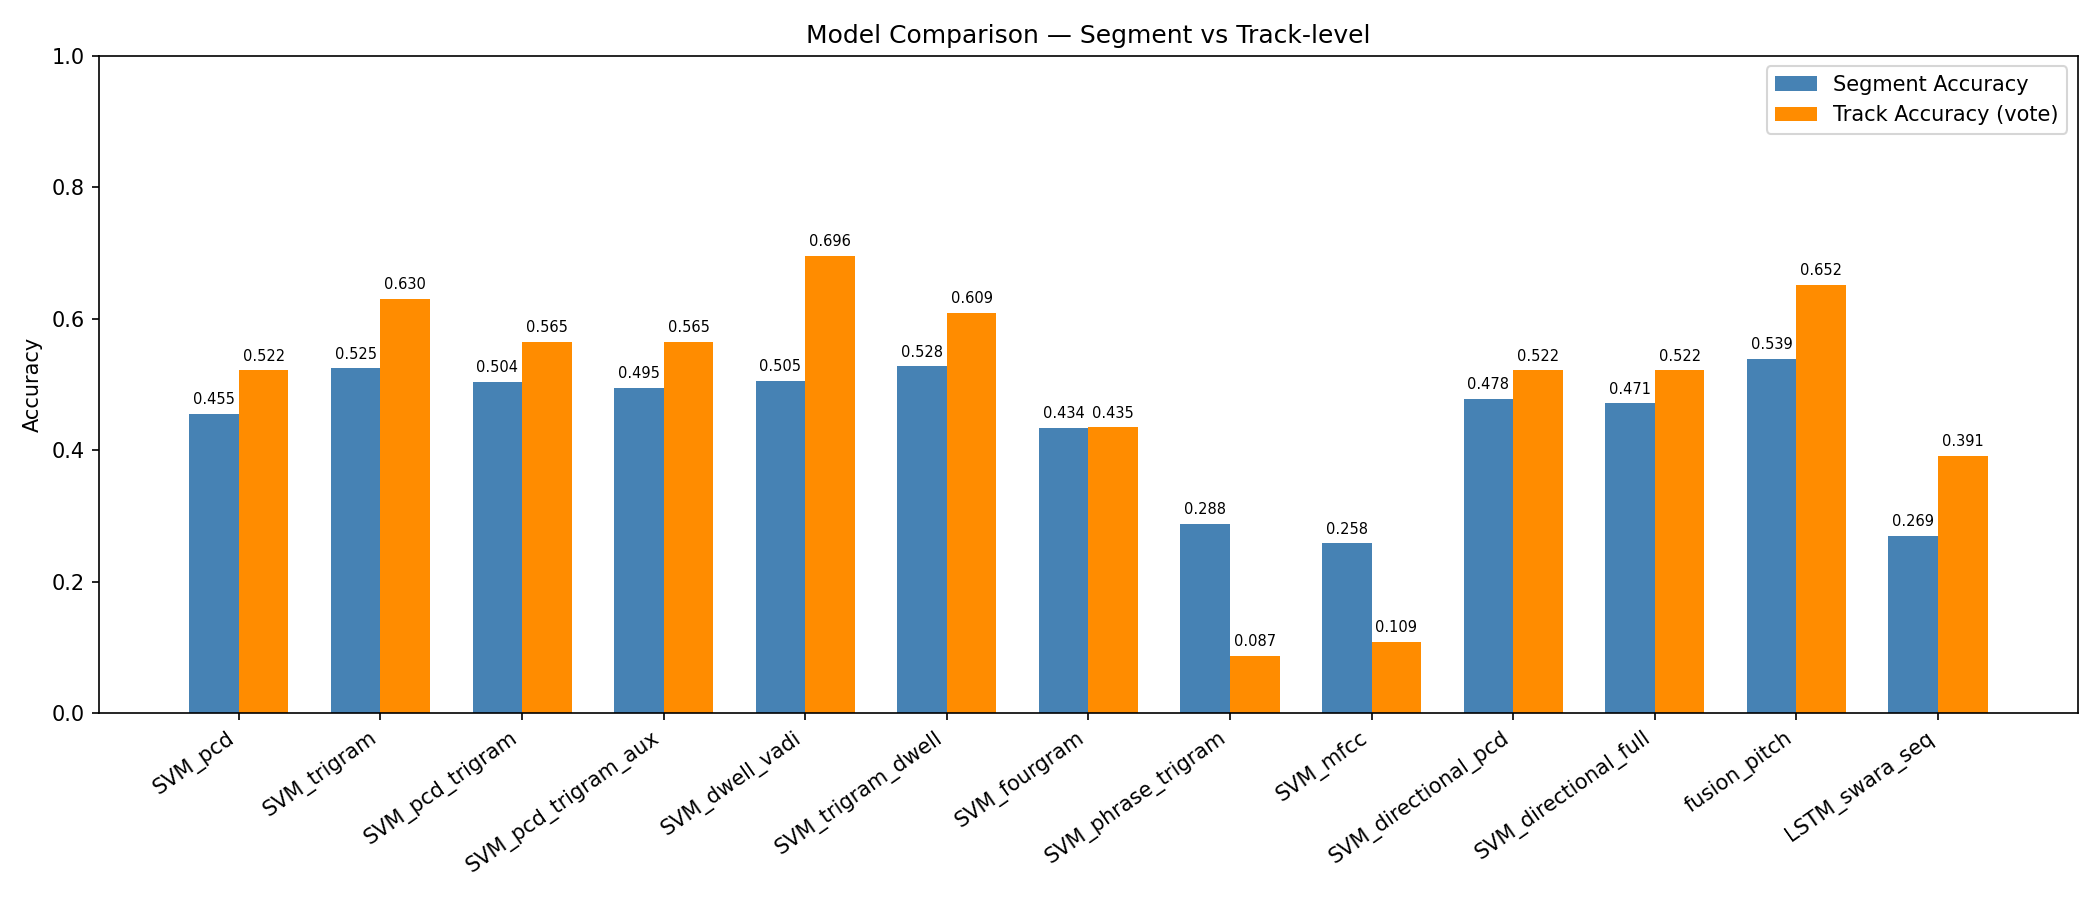
\includegraphics[width=0.85\textwidth]{outputs/figures/classification/excl-est/model_comparison.png}
\caption{Segment and track accuracy across all feature sets. Dwell\_vadi (16d) achieves the highest track accuracy despite being the most parsimonious representation; MFCC scores near random chance.}
\label{fig:model-comparison}
\end{figure}

\subsection{Hypothesis-Driven Analysis}
\label{sec:hypotheses}

Six hypotheses were formulated before experimentation to link classification results to cognitive predictions. Five are confirmed and one yields an informative negative result.

\textbf{H1: Trigrams encode pakad.} Trigram (200d) achieves 52.49\% segment accuracy, outperforming PCD (120d) at 45.51\% by 7.0 percentage points. The gap demonstrates that sequential order matters: PCD captures which notes appear, but trigrams capture in which patterns they occur. Combined with dwell-time (trigram\_dwell, 216d), accuracy reaches 52.79\%. This confirms that characteristic phrase recognition is a primary computational cue, consistent with Saffran et al.~\cite{saffran1999}'s demonstration that transition probability statistics are sufficient for segmenting auditory streams.

\textbf{H2: \textit{Raga} is structural, not timbral.} MFCC achieves 4.39\% track F1w---near chance---and 63 percentage points below dwell\_vadi (67.80\%) under the identical SVM pipeline. The only difference is the input features. This is computational evidence for the modular architecture proposed by Peretz and Coltheart~\cite{peretz2003}: \textit{raga} identity resides in the pitch organisation pathway, not the timbre pathway. All subsequent MFCC results in this report confirm this finding across conditions (Section~\ref{sec:tonic-ablation}) and \textit{raga} set sizes (Section~\ref{sec:perraga}).

\textbf{H3: Cognitive parsimony.} The most parsimonious feature set (dwell\_vadi, 16d) achieves the highest track F1w (67.80\%), outperforming every higher-dimensional alternative: trigram\_dwell (216d) at 57.20\%, pcd\_trigram (320d) at 51.89\%, and directional\_pcd (408d) at 49.08\%. Performance degrades with added dimensions beyond the cognitively motivated core. This mirrors the less-is-more effect described by Gigerenzer et al.~\cite{gigerenzer1999}: in noisy, low-data environments, focused representations outperform exhaustive ones.

\textbf{H4: Confusion follows melakarta kinship.} A permutation test (10,000 iterations) confirms that within-family confusion (16.49\%) is $5.19\times$ higher than between-family confusion (3.18\%), with $p < 0.0001$. The Harik\=ambh\=oji family shows the strongest effect: K\=a\d{m}bh\=oji$\rightarrow$Harik\=ambh\=oji confusion reaches 36.4\%, and Kam\=as$\rightarrow$Harik\=ambh\=oji reaches 21.9\% (both from the 28th melakarta family). This is consistent with the \textit{raga} similarity space found by Castellano et al.~\cite{castellano1984}, where \textit{ragas} sharing a parent scale cluster together perceptually. The family-annotated confusion matrix and permutation test visualisation are in the Appendix (G.3, Figure~25).

\begin{figure}[ht]
\centering
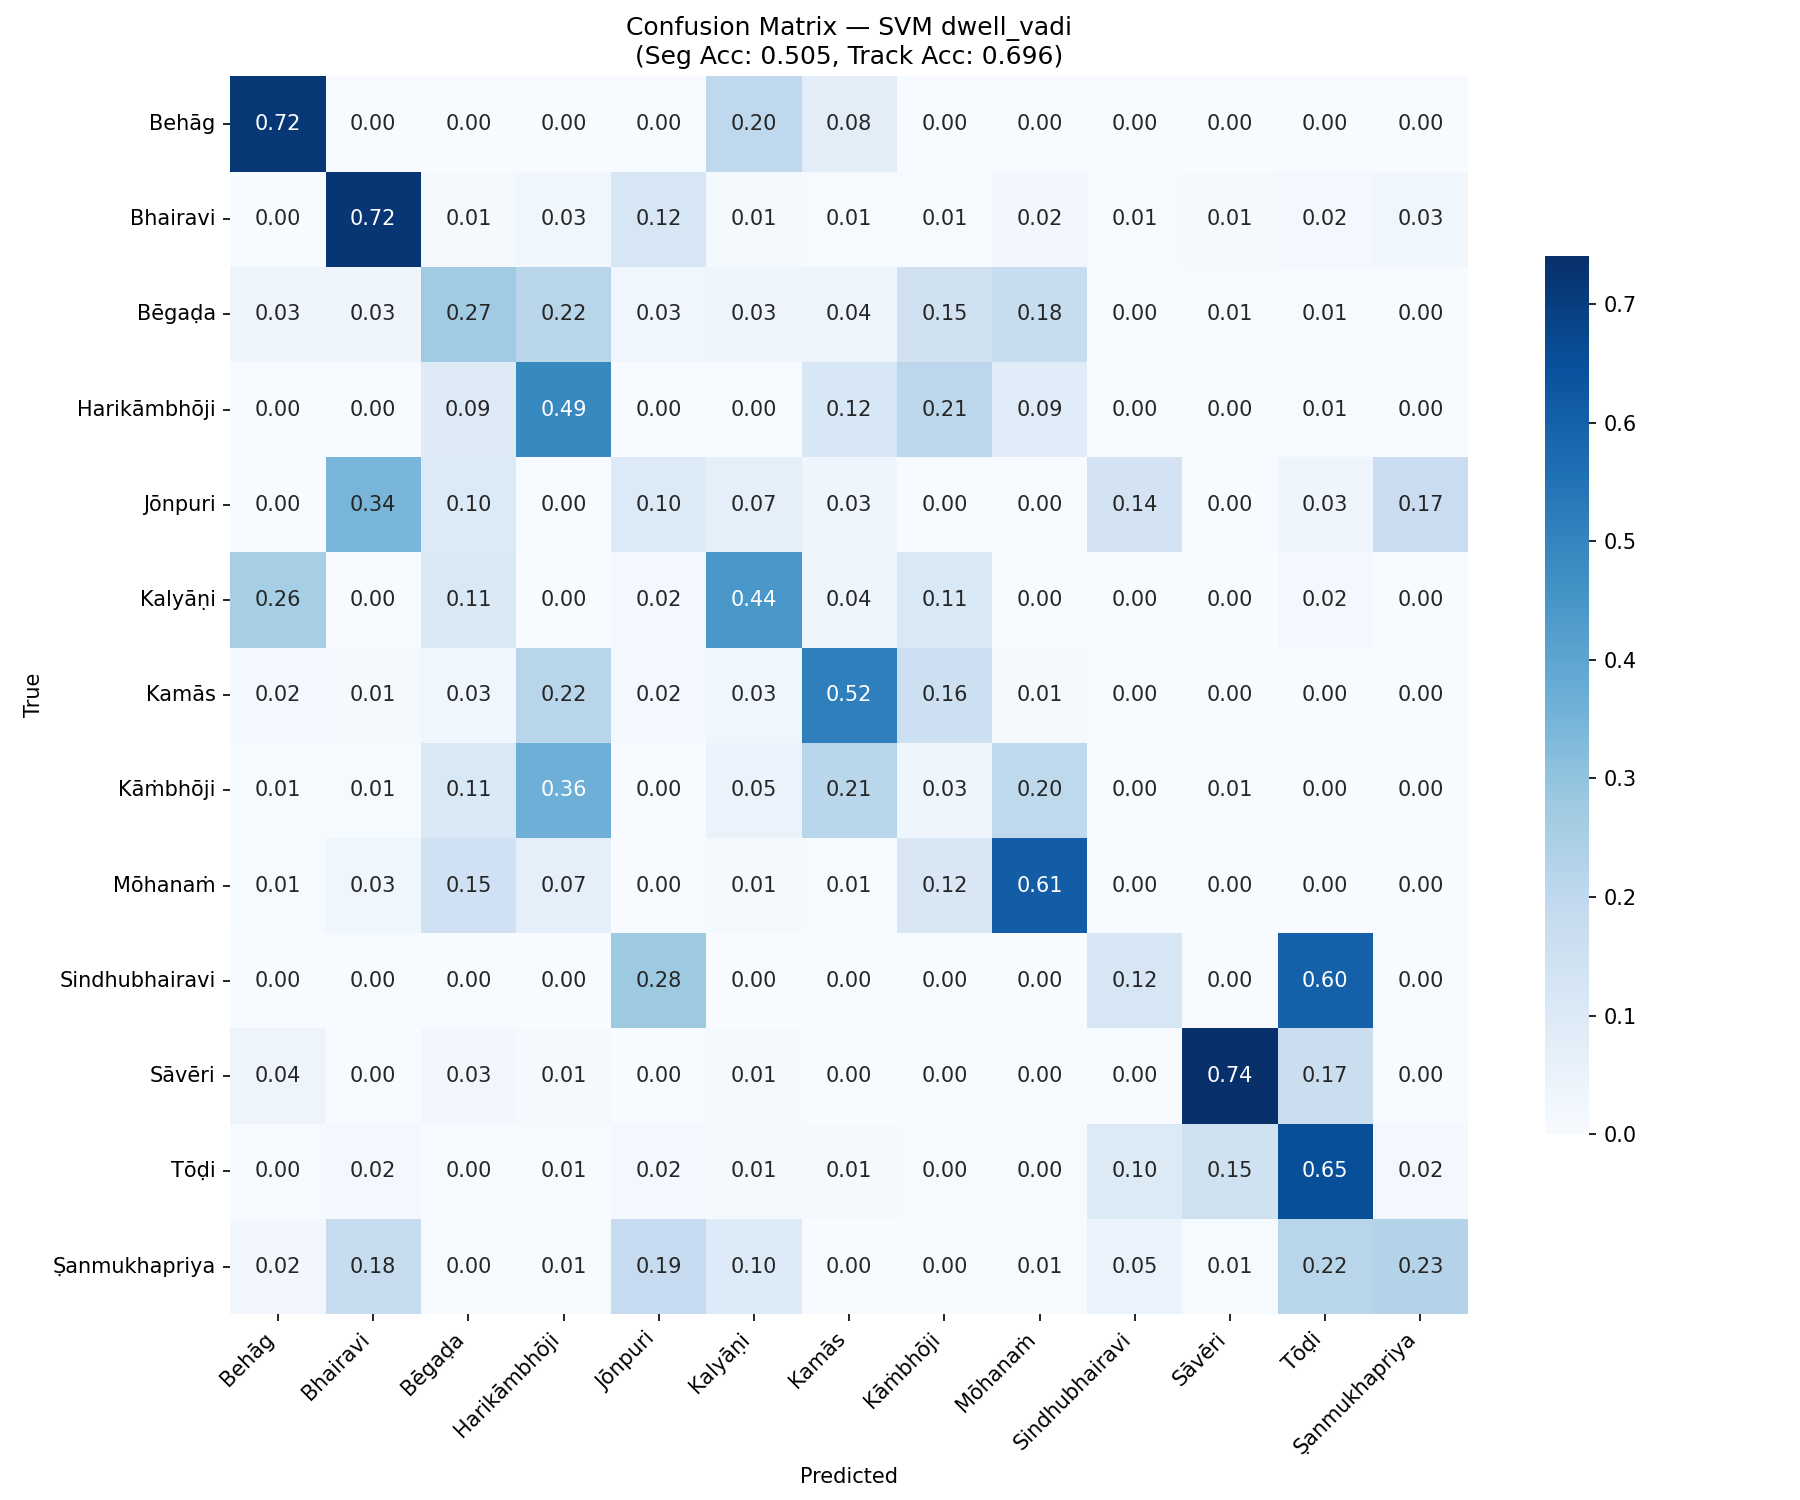
\includegraphics[width=0.48\textwidth]{outputs/figures/classification/excl-est/cm_SVM_dwell_vadi.png}
\hfill
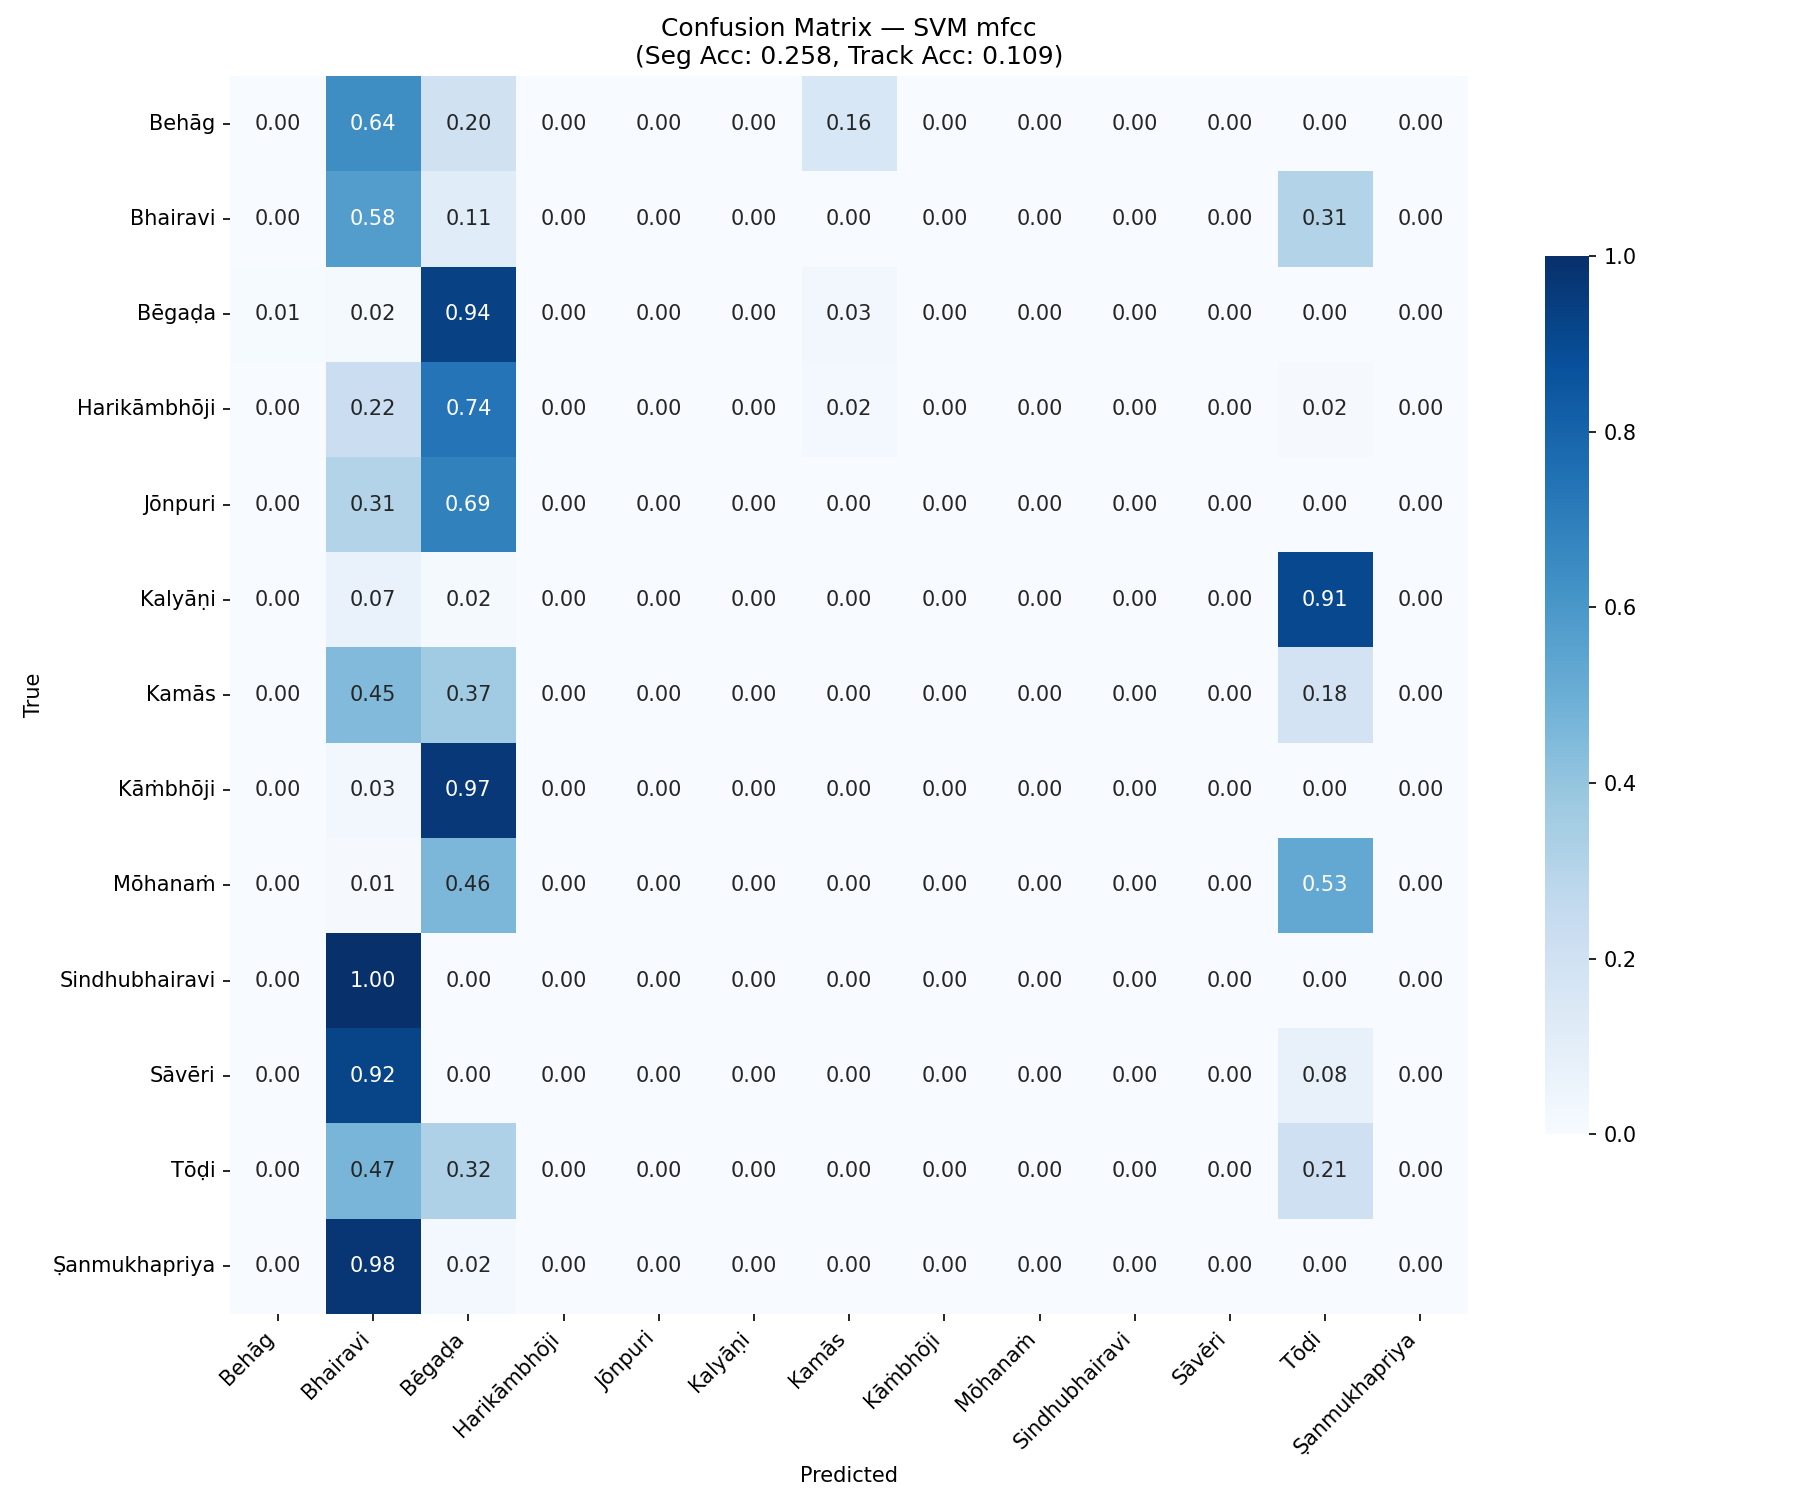
\includegraphics[width=0.48\textwidth]{outputs/figures/classification/excl-est/cm_SVM_mfcc.png}
\caption{Confusion matrices for dwell\_vadi (left, 67.8\% track F1w) and MFCC (right, 4.4\% track F1w). Dwell\_vadi shows a clear diagonal with within-family confusion (Harik\=ambh\=oji cluster), while MFCC produces near-random predictions, confirming that \textit{raga} identity is structural, not timbral (H2).}
\label{fig:confusion-matrices}
\end{figure}

\textbf{H5: Dwell-time captures v\=adi emphasis.} Just 16 features achieve 67.80\% track F1w---$8.8\times$ above random chance---and outperform every other representation at track level. This provides computational validation of Castellano et al.~\cite{castellano1984}'s finding that tone duration distributions predict listener ratings of tonal stability. Dwell\_vadi gains 16 percentage points in F1w from segment-to-track majority voting (51.36\%$\rightarrow$67.80\%), compared to 7 for trigram\_dwell---the mechanism is that dwell-time errors under a noisy tonic are random and correctable by voting, while trigram errors are systematic (Section~\ref{sec:tonic-ablation} quantifies this).

\textbf{H6: Directional encoding is uninformative (Informative negative).} Directional PCD (408d: 47.82\% segment) performs worse than plain trigrams (200d: 52.49\%). Three factors explain this: gamakas blur the ascending/descending distinction at this extraction granularity; trigrams already encode direction implicitly; and doubling the feature space increases sparsity without proportional information gain. The \=arohana/avarohana distinction, while central to \textit{raga} grammar, does not decompose cleanly in performed Carnatic music due to gamaka~\cite{krishnaswamy2003}.

\subsection{Negative Results and Failed Experiments}
\label{sec:negative}

The most informative failure was phrase-aware trigrams: splitting swara sequences at glide boundaries collapsed track F1w to 2.80\% (below chance), demonstrating that Carnatic gamakas connect notes across phrase boundaries rather than separating them~\cite{krishnaswamy2003}---a Western-music intuition about phrase segmentation actively destroys Carnatic melodic information. 4-grams (top-200 vocabulary, same as trigrams) achieved only 38.79\% track F1w despite identical dimensionality to trigrams (both 200d; trigram achieves 59.14\%), confirming that longer n-grams are too sparse with ${\sim}1{,}600$ training segments. The BiLSTM (36.39\% track F1w) suffers from data starvation, and hierarchical melakarta routing did not improve over the flat baseline because 60.7\% of errors are within-family (where L1 routing cannot help). Confusion matrices for gamaka features, 4-grams, phrase trigrams, and the hierarchical vs flat comparison are in the Appendix (G.4, Figures~26--28).

\subsection{Tonic Source Ablation}
\label{sec:tonic-ablation}

\begin{table}[ht]
\centering
\caption{Effect of tonic source on classification accuracy and weighted F1. Feature rankings are preserved across all three conditions.}
\label{tab:tonic}
\small
\begin{tabular}{@{}lrrrrrrr@{}}
\toprule
 & & \multicolumn{3}{c}{\textbf{trigram\_dwell}} & \multicolumn{2}{c}{\textbf{dwell\_vadi}} \\
\cmidrule(lr){3-5} \cmidrule(lr){6-7}
\textbf{Condition} & \textbf{Tracks} & \textbf{Seg F1w} & \textbf{Trk Acc} & \textbf{Trk F1w} & \textbf{Trk Acc} & \textbf{Trk F1w} \\
\midrule
Ground truth & 53 & 59.50\% & 58.49\% & 54.90\% & 52.83\% & 52.70\% \\
Estimated (bad excluded) & 46 & 50.41\% & 60.87\% & 57.20\% & 69.57\% & 67.80\% \\
Estimated (all tracks) & 53 & 41.46\% & 56.60\% & 56.21\% & 50.94\% & 45.21\% \\
\bottomrule
\end{tabular}

\smallskip
\footnotesize{Full per-model results for estimated tonic (all tracks) are in the Appendix (G.5, Table~4). Ground-truth tonic results are in Section~G.6 (Table~5).}
\end{table}

Tonic estimation error, not feature design, is the primary bottleneck: a wrong tonic shifts every swara label by a fixed interval---Sa becomes Ri, Ri becomes Ga---producing an entirely fictitious melodic grammar that bears no relation to the actual \textit{raga}. Three scoring functions were evaluated (Figure~\ref{fig:tonic-methods}); the harmonic method was selected for its combination of highest accuracy (82.2\%) and lowest octave error rate (20.5\%). Removing 13 mis-estimated tracks (18\% of the dataset) recovers most accuracy. Feature rankings are preserved across all conditions, validating the methodology independently of tonic quality. MFCC remains near chance regardless of tonic source, confirming H2.

\begin{figure}[ht]
\centering
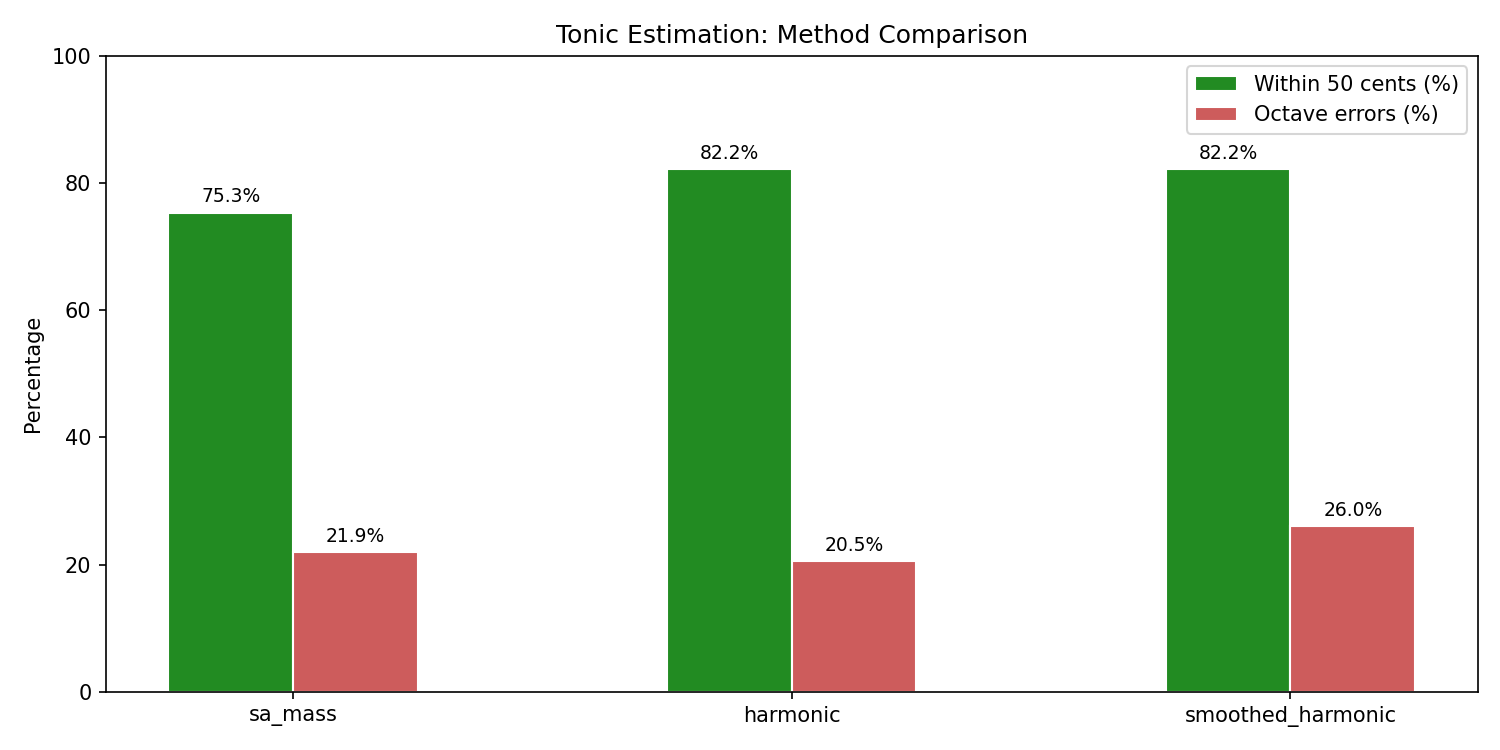
\includegraphics[width=0.75\textwidth]{outputs/figures/tonic_validation/tonic_method_comparison.png}
\caption{Tonic estimation method comparison. The harmonic scoring function achieves 82.2\% accuracy within 50 cents with the lowest octave error rate (20.5\%), motivating its selection as the primary tonic estimator.}
\label{fig:tonic-methods}
\end{figure}

Notably, dwell\_vadi achieves the highest track accuracy under estimated tonic with bad-tonic exclusion (69.57\% vs trigram\_dwell at 60.87\%). The mechanism: a mis-estimated tonic shifts all swara labels by a fixed interval, but the \emph{relative duration ranking} is preserved---the note held longest is still held longest, just under a different label. These random label errors are correctable by majority voting across segments (dwell\_vadi gains 19 percentage points from segment to track). Trigram errors, by contrast, are systematic: a shifted tonic produces consistently wrong three-note sequences across every segment, and voting amplifies rather than corrects the error.

\subsection{Per-\textit{Raga} Case Studies}
\label{sec:perraga}

Per-\textit{raga} F1 scores correlate with musical distinctiveness, not data quantity: T\=o\d{d}i (0.86 F1, 6 tracks) far outperforms Kam\=as (0.36 F1, 7 tracks) because it has a unique intervallic signature, while Kam\=as shares its trigram vocabulary with the Harik\=ambh\=oji family (per-\textit{raga} pitch class distributions and transition matrices illustrating this contrast are in the Appendix). Excluding the four most ambiguous Harik\=ambh\=oji-family \textit{ragas}, trigram\_dwell reclaims the top position at 70.0\% track accuracy, with the feature ranking inverting: trigrams lead dwell\_vadi by 5 percentage points, suggesting dwell-time is more robust to ambiguous \textit{ragas} while trigrams are more discriminative once genuinely distinct \textit{ragas} dominate.

% ── 5. Discussion, Limitations and Future Work ──────────
\section{Discussion, Limitations, and Future Work}

\subsection{Interpreting the Results}

Published \textit{raga} recognition systems report 80--96\% accuracy, but most use train/test splits without cross-performance validation and operate on Hindustani music where gamaka density is lower. Under equivalent methodological constraints---GroupKFold evaluation, Carnatic repertoire with dense gamaka, polyphonic audio without source separation, and estimated tonic---67\% track accuracy with fully interpretable features represents a meaningful baseline. The SVM's advantage over the BiLSTM (over 30 percentage points at track level) reflects data regime rather than architectural superiority: hand-crafted features encode the invariances that the LSTM must discover from raw sequences; with 1,648 segments across 13 classes, the SVM's inductive bias is better matched.

The six hypotheses, taken together, tell a coherent story. H1--H5 confirm that the features cognitive theory predicts listeners rely on---characteristic phrase patterns (trigrams) and note prominence hierarchies (dwell-time)---are the same features that achieve the best classification performance. This alignment is not circular: the features were designed \textit{before} classification, based on published perceptual evidence, and the hypotheses were formulated before experimentation. The one failure (H6) is equally informative: directional encoding does not improve accuracy because gamaka blurs the ascending/descending distinction in performed Carnatic music~\cite{krishnaswamy2003}, exactly as musicological theory would predict. The system's errors are as interpretable as its successes.

The Harik\=ambh\=oji family exhibits the strongest within-family ambiguity, with sibling \textit{ragas} sharing identical note sets and differing only in gamaka contour, precisely the continuous pitch information that the token collapse step discards. Rather than undermining the system, this confusion validates its interpretability: we can trace \textit{why} the classifier struggles, and the reason is musicologically coherent.

\subsection{Limitations}

The most consequential limitation is tonic estimation quality: the 18\% tonic failure rate (13 of 73 tracks) propagates through every downstream stage and represents the pipeline's hard ceiling. Multiple alternative strategies were explored (harmonic triad scoring, ensemble methods, segment-level voting, source separation via Demucs and HPSS) but none surpassed 82.2\%, confirming that polyphonic audio without vocal isolation represents a hard limit.

The dataset is small (73 tracks, 13 \textit{ragas} after filtering) with substantial class imbalance (14.6:1). The system has been evaluated on a single dataset (SARAGA Carnatic) with no external validation corpus, and the cognitive claims rest on feature-performance correlations rather than direct behavioural experiments with human listeners. Finally, the equal-tempered 100-cent swara bins impose a Western tuning grid on a tradition that uses \textit{raga}-specific intonation, potentially losing fine-grained pitch distinctions.

\subsection{Future Work}

Source separation remains the most impactful potential improvement: effective vocal isolation would lift the tonic estimation ceiling and unlock the remaining 18\% of tracks currently excluded. Gamaka-aware features preserving continuous pitch contour information (e.g., pitch slope distributions, vibrato parameters) could address within-family disambiguation, directly targeting the Harik\=ambh\=oji failure described above.

A preliminary cross-tradition test on 10 Hindustani tracks revealed a striking feature-importance flip: dwell\_vadi dominated while trigrams collapsed---consistent with Hindustani music being emphasis-driven rather than phrase-driven (model comparison, confusion matrix, and swara mapping for the Hindustani pilot are in the Appendix~H.3, Figures~29--30). With a larger Hindustani corpus, this could test whether the cognitive mechanisms that drive \textit{raga} recognition differ systematically between traditions. Expanding to larger and more diverse datasets would also strengthen the generalisability of the current findings. Finally, validating the feature hierarchy against behavioural data from human listeners would strengthen the cognitive claims from correlation to direct evidence.

% ── 6. Conclusion ─────────────────────────────────────────
\section{Conclusion}

The answer to the research question is a qualified yes. This project has shown that features designed to mirror cognitive mechanisms, trigrams encoding statistical learning of characteristic phrases and dwell-time profiles encoding tonal hierarchies that listeners rate as structurally important, outperform both timbral baselines and a deep learning alternative under rigorous cross-performance evaluation. The inferential step from ``cognitively motivated features work best'' to ``the pipeline mirrors cognition'' rests not on any single accuracy figure, but on the coherence of six hypothesis tests and five negative results whose failures are as theoretically interpretable as the successes.

The practical contribution is a 16-dimensional dwell-time representation achieving 67.8\% weighted F1 (69.6\% track accuracy) on 13 \textit{ragas}, outperforming a BiLSTM by over 31 percentage points in F1w. In domains where theoretical priors are rich and data is scarce, the choice between interpretability and accuracy is a false dichotomy. The features that music cognition predicts should matter are the features that matter computationally.

% ── References ────────────────────────────────────────────
{\small\setlength{\itemsep}{0pt}\setlength{\parskip}{0pt}
\renewcommand{\refname}{References}
\begin{thebibliography}{20}

\bibitem{burns1978}
E.~M. Burns and W.~D. Ward, ``Categorical perception---phenomenon or epiphenomenon: Evidence from experiments in the perception of melodic musical intervals,'' \textit{Journal of the Acoustical Society of America}, vol.~63, no.~2, pp.~456--468, 1978.

\bibitem{castellano1984}
M.~A. Castellano, J.~J. Bharucha, and C.~L. Krumhansl, ``Tonal hierarchies in the music of North India,'' \textit{Journal of Experimental Psychology: General}, vol.~113, no.~3, pp.~394--412, 1984.

\bibitem{chordia2007}
P.~Chordia and A.~Rae, ``Raag recognition using pitch-class and pitch-class dyad distributions,'' in \textit{Proc. International Society for Music Information Retrieval Conference (ISMIR)}, 2007.

\bibitem{gigerenzer1999}
G.~Gigerenzer, P.~M. Todd, and the ABC Research Group, \textit{Simple Heuristics That Make Us Smart}. Oxford University Press, 1999.

\bibitem{gulati2016}
S.~Gulati, J.~Serr\`a, V.~Ishwar, S.~Sent\"urk, and X.~Serra, ``Phrase-based \textit{raga} recognition using vector space modeling,'' in \textit{Proc. IEEE International Conference on Acoustics, Speech and Signal Processing (ICASSP)}, 2016, pp.~66--70.

\bibitem{kim2018}
J.~W. Kim, J.~Salamon, P.~Li, and J.~P. Bello, ``CREPE: A convolutional representation for pitch estimation,'' in \textit{Proc. IEEE International Conference on Acoustics, Speech and Signal Processing (ICASSP)}, 2018, pp.~161--165.

\bibitem{koduri2012}
G.~K. Koduri, S.~Gulati, P.~Rao, and X.~Serra, ``\textit{Raga} recognition based on pitch distribution methods,'' \textit{Journal of New Music Research}, vol.~41, no.~4, pp.~337--350, 2012.

\bibitem{krishna2012}
T.~M. Krishna and V.~Ishwar, ``Carnatic music: Svara, gamaka, motif and raga identity,'' in \textit{Proc. 2nd CompMusic Workshop}, 2012, pp.~12--18.

\bibitem{krishnaswamy2003}
A.~Krishnaswamy, ``On the twelve basic intervals in South Indian classical music,'' in \textit{Proc. Audio Engineering Society Convention}, 2003.

\bibitem{krumhansl1990}
C.~L. Krumhansl, \textit{Cognitive Foundations of Musical Pitch}. Oxford University Press, 1990.

\bibitem{mauch2014}
M.~Mauch and S.~Dixon, ``pYIN: A fundamental frequency estimator using probabilistic threshold distributions,'' in \textit{Proc. IEEE International Conference on Acoustics, Speech and Signal Processing (ICASSP)}, 2014, pp.~659--663.

\bibitem{pearce2012}
M.~T. Pearce and G.~A. Wiggins, ``Auditory expectation: The information dynamics of music perception and cognition,'' \textit{Topics in Cognitive Science}, vol.~4, no.~4, pp.~625--652, 2012.

\bibitem{peretz2003}
I.~Peretz and M.~Coltheart, ``Modularity of music processing,'' \textit{Nature Neuroscience}, vol.~6, no.~7, pp.~688--691, 2003.

\bibitem{saffran1996}
J.~R. Saffran, R.~N. Aslin, and E.~L. Newport, ``Statistical learning by 8-month-old infants,'' \textit{Science}, vol.~274, no.~5294, pp.~1926--1928, 1996.

\bibitem{saffran1999}
J.~R. Saffran, E.~K. Johnson, R.~N. Aslin, and E.~L. Newport, ``Statistical learning of tone sequences by human infants and adults,'' \textit{Cognition}, vol.~70, no.~1, pp.~27--52, 1999.

\bibitem{singh2024}
P.~Singh and V.~Arora, ``Explainable deep learning analysis for raga identification in Indian art music,'' \textit{arXiv preprint arXiv:2406.02443}, 2024.

\bibitem{srinivasamurthy2021}
A.~Srinivasamurthy, S.~Gulati, R.~Caro Repetto, and X.~Serra, ``Saraga: Open datasets for research on Indian art music,'' \textit{Empirical Musicology Review}, vol.~16, no.~1, pp.~85--98, 2021.

\bibitem{sturm2014}
B.~L. Sturm, ``A simple method to determine if a music information retrieval system is a `horse','' \textit{IEEE Transactions on Multimedia}, vol.~16, no.~6, pp.~1636--1644, 2014.

\bibitem{tillmann2000}
B.~Tillmann, J.~J. Bharucha, and E.~Bigand, ``Implicit learning of tonality: A self-organizing approach,'' \textit{Psychological Review}, vol.~107, no.~4, pp.~885--913, 2000.

\bibitem{viswanathan2004}
T.~Viswanathan and M.~H. Allen, \textit{Music in South India: The Kar\d{n}\=a\d{t}ak Concert Tradition and Beyond}. Oxford University Press, 2004.

\end{thebibliography}}

% ── Appendices ────────────────────────────────────────────
\appendix

% Figures removed -- add confusion matrix images here if needed
% \begin{figure}[ht]
% \centering
% 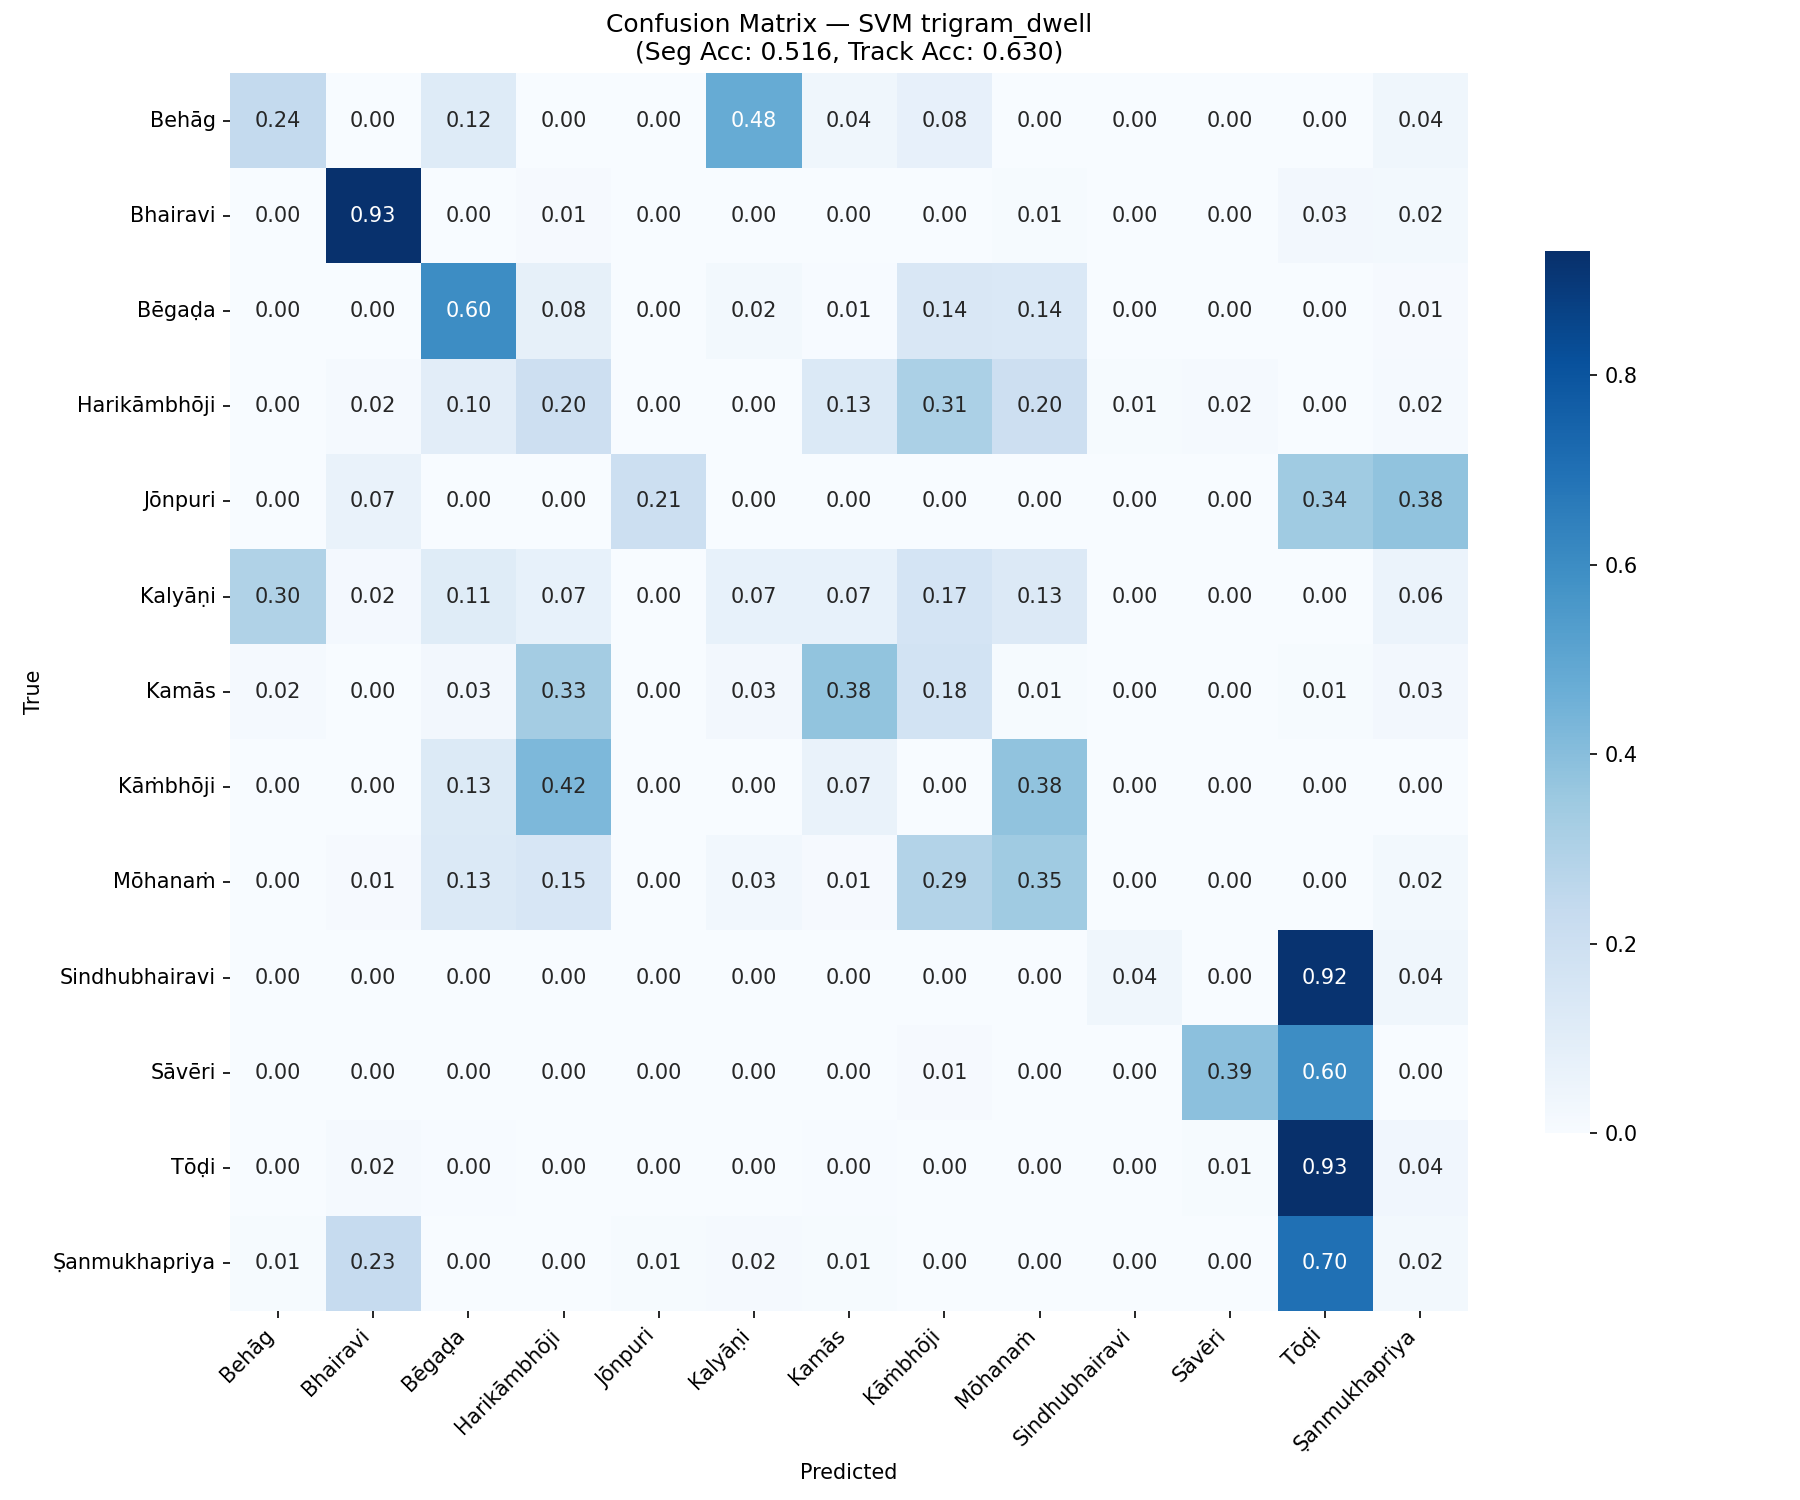
\includegraphics[width=0.8\textwidth]{outputs/figures/classification/cm_SVM_trigram_dwell.png}
% \caption{Confusion matrix for SVM trigram\_dwell (14 \textit{ragas}, estimated tonic, bad-tonic excluded).}
% \label{fig:cm14}
% \end{figure}
%
% \begin{figure}[ht]
% \centering
% \includegraphics[width=0.8\textwidth]{outputs/figures/classification/cm_SVM_trigram_dwell_10raga.png}
% \caption{Confusion matrix for SVM trigram\_dwell (10 \textit{ragas}).}
% \label{fig:cm10}
% \end{figure}


\end{document}